% -- Deckblatt.tex -----------------------------------------------------------
%
%   Gestaltung des Deckblattes der Bedienungsanleitung:  
%   - Einbinden und formatieren der Logos
%   - Bezeichnungen befinden sich in 'Meta.tex'   
% ------------------------------------------------------------------------------

\thispagestyle{empty} % von plain nach empty
\begin{titlepage}
\vspace*{-3cm}% vertikale negative Verschiebung
%%------------------------------------------------------------------------------
%%   Firmenlogo einf�gen
%%------------------------------------------------------------------------------
\begin{figure}[h]
\centering

\includegraphics[width=0.25\textwidth]{schlizbaeda.png}
\end{figure}

\begin{center}
\LARGE{\textbf{\Dokumentart}}\\[1.5ex] 
\Large{\Bezeichnung}\\[4ex]
%%------------------------------------------------------------------------------
%%   Titel der Bedienungsanleitung
%%------------------------------------------------------------------------------
\noindent\rule[1ex]{\textwidth}{3pt} % vertikaler Strich
%\huge{\textbf{\titel}}\\[1.5ex]      % TITEL DER ARBEIT
\textbf{\titel}\\[1.5ex]              % TITEL DER ARBEIT (lange �berschrift)
\noindent\rule[1ex]{\textwidth}{3pt} 
%\LARGE{\textbf{\untertitel}}\\[6ex]
%\LARGE{\textbf{\art}}\\[1.5ex]
%\Large{im Fachgebiet \fachgebiet}
\\[2ex]

\normalsize
%%------------------------------------------------------------------------------
%%   Bild
%%------------------------------------------------------------------------------
\begin{figure}[h]
\centering
%\includegraphics[width=1.0\textwidth]{Schaltschrank.png}
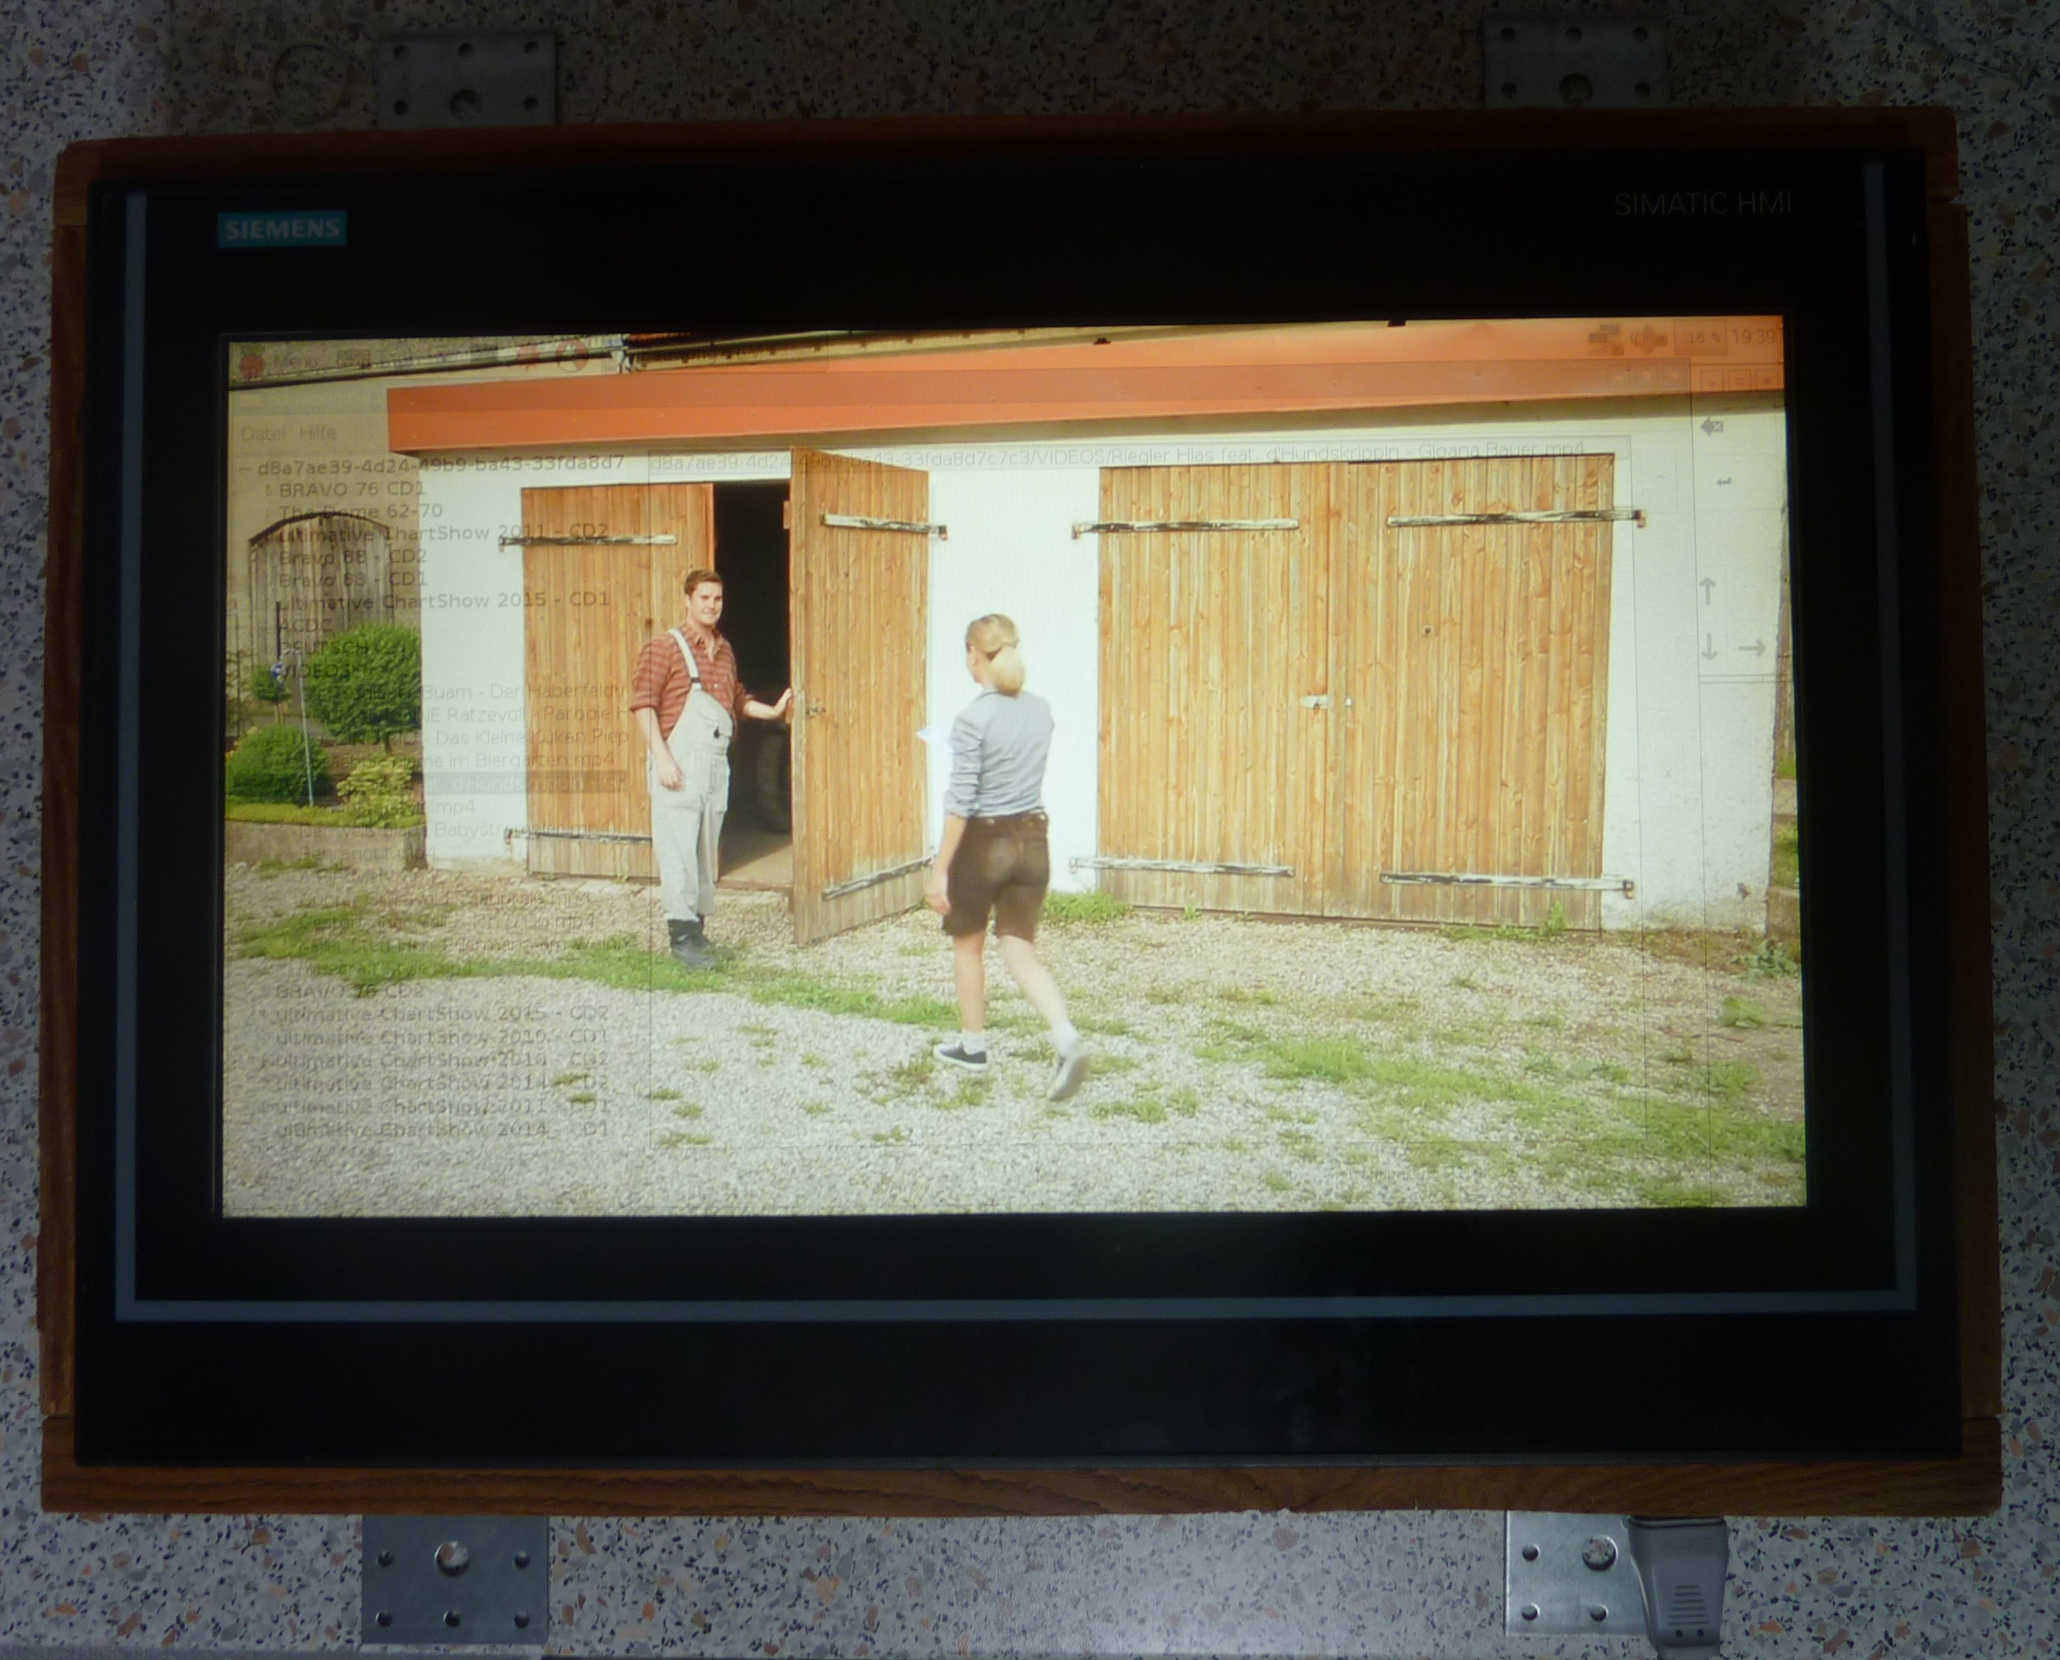
\includegraphics[width=12cm]{Titelbild.jpg}
\end{figure}

%%------------------------------------------------------------------------------
%%   CE und Firmenadresse
%%------------------------------------------------------------------------------
\begin{tabular}{p{6cm} p{6cm} p{2cm}}\\
\hline
% --- Zeile mit dem offiziellen Logo der Free Software Foundation:
%\parbox[c]{1em}{\includegraphics[width=1in]{CE.png}} & PAK GmbH, Pf<E4>lzerstra<DF>e 1\newline D-83109 Gro<DF>karolinenfeld   & Datum:\newline 07.11.2014\\
\parbox[c]{1em}{
\includegraphics[width=1in]{GPLv3_Logo.png}} & GNU General Public License v3 \newline \copyright\ \jahr\ \autor & Datum:\newline 01.07.2016\\ %{\includegraphics[width=1in]{Official_gnu.png}}\\
%\parbox[c]{1em}{\includegraphics{Official_gnu.png}} {\Bezeichnung} -- {\BezeichnungLang} {\Version}\newline (C) 2016 schlizbaeda, GNU GPL v3 & Datum:\newline 20.02.2016
% --- Zeile ohne CE-Zeichen:
%\parbox[c]{0em} \ PAK GmbH & Pf�lzerstra�e 1\newline D-83109 Gro�karolinenfeld   & Datum:\newline 07.11.2014\\

\hline
\end{tabular}
\\[4ex]

%\copyright\ \jahr\\

%\includegraphics[width=1in]{EQM_Zert.png}
\end{center}

\textbf{}\\
\textbf{}\\
Die Abbildung auf dem Display stammt aus dem Video zu folgendem Musikst�ck:\\
\texttt{\textbf{Riegler Hias feat. d' Hundskrippln} \textit{Gloana Bauer}} bei 2:42\\
\url{http://www.hundskrippln.de/#filme} %-- 2:42


\end{titlepage}



